\documentclass[11pt]{article}

\usepackage[margin=1in]{geometry}
\usepackage{amsmath,amssymb,amsthm}
\usepackage{graphicx}
\usepackage[colorlinks=true,linkcolor=blue,citecolor=blue,urlcolor=blue]{hyperref}

\newtheorem{theorem}{Theorem}
\newtheorem{corollary}{Corollary}
\newtheorem{lemma}{Lemma}

\DeclareMathOperator{\Id}{Id}
\DeclareMathOperator{\dist}{d}

\title{A Common Quotient-Subspace Obstruction to the Real HFP Conjecture}
\author{FA/Banach smoke run \texttt{fa\_banach\_001}}
\date{2026-06-14}

\begin{document}
\maketitle

\section*{Status}

This is a candidate partial result for Conjecture 5.2 of Aubrun and
Muller-Hermes, \emph{Limit formulas for norms of tensor power operators},
arXiv:2410.23063. It proves a common quotient-subspace obstruction to the
Hilbert space factorization property (HFP). It does not solve the full
conjecture.

\section*{Source Question}

Aubrun and Muller-Hermes define a pair $(X,Y)$ of Banach spaces to have the
HFP if every bounded operator $\phi:X\to Y$ satisfies
\[
  \gamma_2(\phi)=\|\phi\|,
\]
where $\gamma_2$ is the factorization norm through Hilbert space. They
conjecture in the real case:

\begin{quote}
  A pair $(X,Y)$ of real Banach spaces has the HFP if and only if $X$ or $Y$
  is a Hilbert space.
\end{quote}

The source records this as Conjecture 5.2 and gives an equivalent
two-dimensional convex-body formulation as Conjecture 5.5.

\begin{center}
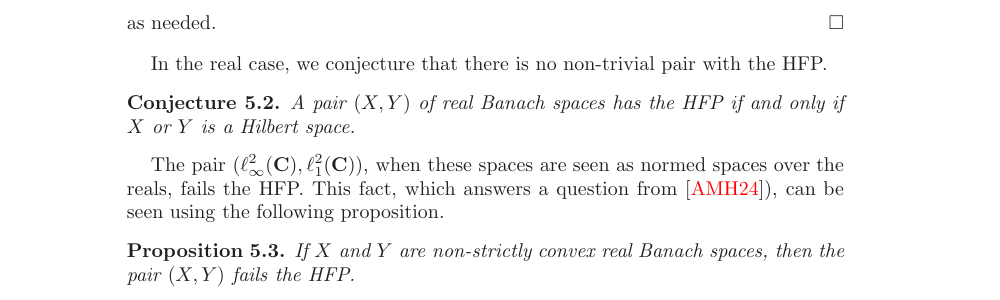
\includegraphics[width=0.92\linewidth]{figures/hfp_conjecture_crop.png}
\end{center}

\begin{center}

\includegraphics[width=0.92\linewidth]{figures/open_problem_crop.png}
\end{center}

\section*{Definitions}

For a bounded operator $u:E\to F$, $\gamma_2(u)$ is
\[
  \inf \{\|a\|\,\|b\| : u=b a,\ a:E\to H,\ b:H\to F,\ H \text{ Hilbert}\}.
\]
If no such factorization exists, $\gamma_2(u)=\infty$.

For an $n$-dimensional Banach space $E$, the Banach-Mazur distance from $E$
to Euclidean space is
\[
  d(E,\ell_2^n)=\inf\{\|S\|\,\|S^{-1}\|: S:E\to \ell_2^n
  \text{ is an isomorphism}\}.
\]

\section*{Proof Intuition}

The source proves that HFP descends to quotients of the domain and subspaces
of the range. Therefore, if a pair $(X,Y)$ had HFP and the same
finite-dimensional non-Hilbert space $E$ appeared both as a quotient of $X$
and as a subspace of $Y$, then $(E,E)$ would also have HFP. But the identity
operator on $E$ has Hilbert factorization norm exactly equal to the
Banach-Mazur distance from $E$ to Euclidean space. This distance is strictly
larger than one when $E$ is not Hilbertian, whereas $\|\Id_E\|=1$.

\begin{lemma}\label{lem:identity}
Let $E$ be an $n$-dimensional real Banach space. Then
\[
  \gamma_2(\Id_E)=d(E,\ell_2^n).
\]
Consequently, if $E$ is not linearly isometric to a Hilbert space, then
$\gamma_2(\Id_E)>1=\|\Id_E\|$.
\end{lemma}

\begin{proof}
If $\Id_E=ba$ factors through a Hilbert space $H$, then $a:E\to H$ is
injective and $b|_{a(E)}=a^{-1}$. Hence
\[
  \|a\|\,\|b\|\geq \|a\|\,\|a^{-1}:a(E)\to E\|.
\]
Since $a(E)$ is an $n$-dimensional Hilbert space, the right-hand side is at
least $d(E,\ell_2^n)$. Taking the infimum over all Hilbert factorizations
gives $\gamma_2(\Id_E)\geq d(E,\ell_2^n)$.

Conversely, any isomorphism $S:E\to \ell_2^n$ gives the factorization
\[
  \Id_E = S^{-1}S
\]
through the Hilbert space $\ell_2^n$, so
$\gamma_2(\Id_E)\leq \|S\|\,\|S^{-1}\|$. Taking the infimum over $S$ gives
the reverse inequality.

Finally, in finite dimension $d(E,\ell_2^n)=1$ holds exactly when the unit
ball of $E$ is an ellipsoid, i.e. when $E$ is Hilbertian. Thus non-Hilbertian
$E$ has $d(E,\ell_2^n)>1$.
\end{proof}

\begin{theorem}\label{thm:main}
Let $X$ and $Y$ be real Banach spaces. Suppose that there is a finite-
dimensional non-Hilbert real Banach space $E$ such that $E$ is linearly
isometric to a quotient of $X$ and linearly isometric to a subspace of $Y$.
Then the pair $(X,Y)$ fails the HFP.
\end{theorem}

\begin{proof}
Assume for contradiction that $(X,Y)$ has HFP. Proposition 5.4 of
Aubrun--Muller-Hermes says that HFP is inherited by quotients of the domain
and subspaces of the range: if $(X,Y)$ has HFP, then $(X/F,Z)$ has HFP for
every quotient $X/F$ of $X$ and every subspace $Z$ of $Y$.

By the hypothesis, choose $F\subset X$ and $Z\subset Y$ so that both $X/F$
and $Z$ are linearly isometric to $E$. Transporting the structure through
these isometries, the pair $(E,E)$ has HFP. Applying HFP to the identity
operator on $E$ gives
\[
  \gamma_2(\Id_E)=\|\Id_E\|=1.
\]
This contradicts Lemma~\ref{lem:identity}, since $E$ is not Hilbertian.
Therefore $(X,Y)$ cannot have HFP.
\end{proof}

\begin{corollary}
If $E$ is a finite-dimensional real Banach space that is not Hilbertian, then
the diagonal pair $(E,E)$ fails HFP.
\end{corollary}

\begin{proof}
Apply Theorem~\ref{thm:main} with $X=Y=E$.
\end{proof}

\begin{corollary}[Two-dimensional convex-body formulation]
Let $K$ and $L$ be centrally symmetric convex bodies in $\mathbb R^2$. If
$K$ and $L$ are linearly equivalent and one of them is not an ellipse, then
the hypothesis of Conjecture 5.5 in the source paper fails for this pair.
\end{corollary}

\begin{proof}
Let $T$ be a linear isomorphism with $T(K)=L$. If the hypothesis of
Conjecture 5.5 held, there would be an ellipse $\mathcal E$ such that
\[
  L=T(K)\subset \mathcal E\subset L.
\]
Thus $\mathcal E=L$, which is impossible unless $L$ is an ellipse. Since
linear equivalence preserves being an ellipse, this contradicts the
assumption that one of $K,L$ is not an ellipse.
\end{proof}

\section*{Verification Notes}

No computation is used. The proof has two dependencies:
\begin{itemize}
  \item the source paper's inheritance proposition for HFP under quotients of
  the domain and subspaces of the range;
  \item the standard identification of $\gamma_2(\Id_E)$ with the
  Banach-Mazur distance from $E$ to Euclidean space.
\end{itemize}
Both are exact norm statements, so no limiting or approximation step is hidden
in the finite-dimensional obstruction.

\section*{Limitations}

The theorem only applies when the same finite-dimensional non-Hilbert space
appears as a quotient of $X$ and as a subspace of $Y$. Conjecture 5.2 remains
open for arbitrary unrelated non-Hilbert pairs.

\section*{Novelty And Search Bounds}

Before packaging, the run's cheap indexes were searched for arXiv:2410.23063,
HFP, Hilbert space factorization, nuclear tensorization, tensor power
operators, and the convex-body ellipse formulation. A local corpus search for
the exact HFP/NTP terminology found the source paper and the earlier
Aubrun--Muller-Hermes tensor-power paper. A bounded web search for the exact
real HFP conjecture language did not reveal a later answer. The source paper
already proves the non-strictly convex pair obstruction and the reduction to
dimension two; this packet records only the common quotient-subspace
obstruction above.

\section*{References}

\begin{itemize}
  \item Guillaume Aubrun and Alexander Muller-Hermes, \emph{Limit formulas
  for norms of tensor power operators}, arXiv:2410.23063.
  \item Joe Diestel, Hans Jarchow, and Andrew Tonge, \emph{Absolutely Summing
  Operators}, Cambridge Studies in Advanced Mathematics 43, Cambridge
  University Press, 1995.
\end{itemize}

\section*{Human Review Recommendation}

Review as a small partial result. The main points to check are the application
of the source inheritance proposition and the equality
$\gamma_2(\Id_E)=d(E,\ell_2^n)$.

\end{document}

